\section{Gated Recurrent Unit}
\label{chap:Gated Recurrent Unit}

  %%%%%%%%%%%%%%%%%%%%%%%%%%%%
  % SUBSECTION               %
  %%%%%%%%%%%%%%%%%%%%%%%%%%%%
\subsection{Brief Intro.}
Gated recurrent units are designed in a
manner to have more persistent memory thereby making it easier for
RNNs to capture long-term dependencies also it is simplified  LSTM cell with less parameters.
\subsection{Inside GRU Cell}
\begin{figure}[H]%
    \center%
    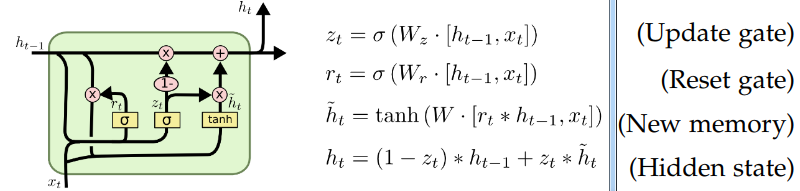
\includegraphics[width=\textwidth]{images/amir/Capture1.png}%
     % you need to add the caption for the list of figures
    \caption[This is gru-inside image]{a look inside GRU cell}\label{fig:gru inside}%
  \end{figure}
\indent$\bullet$Update Gate: The update signal $z_t$
is responsible for determining
how much of $h_{t-1}$ should be carried forward to the next state. For
instance, if $z_{t} \approx 1$, then  $h_{t-1}$ is almost entirely copied out to ht
.
Conversely, if $z_{t} \approx 0$, then mostly the new memory $\tilde{h}_{t}$ 
is forwarded
to the next hidden state.\\
\indent$\bullet$Reset Gate: The reset signal $r_t$
is responsible for determining how
important $h_{t-1}$ is to the summarization $\tilde{h}_{t}$
. The reset gate has the
ability to completely diminish past hidden state if it finds that $h_{t-1}$
is irrelevant to the computation of the new memory.\\
\indent$\bullet$New memory generation: A new memory $\tilde{h}_{t}$
is the consolidation of
a new input word $x_t$ with the past hidden state $h_{t-1}$. Anthropomorphically,
this stage is the one who knows the recipe of combining a
newly observed word with the past hidden state $h_{t-1}$ to summarize
this new word in light of the contextual past as the vector $\tilde{h}_{t}$ .\\
\indent$\bullet$Hidden state: The hidden state $h_t$
is finally generated using the
past hidden input $h_{t-1}$ and the new memory generated $\tilde{h}_{t}$ with the
advice of the update gate.\\
\subsection{LSTM vs GRU – Who wins?}
There has been a lot of debate around which among the two wins without an objective answer yet. Here are a few widely accepted principles:\\
GRU runs a lot faster because of the lower number of parameters so they might take lesser time to train and generalize. GRU is much younger than LSTM. Bidirectional GRU performance does not deteriorate from moving left to right like LSTM.\\
To sum up, GRU has two gates (reset and update gates) whereas an LSTM has three gates (namely input, output and forget gates).



.